\documentclass[a4paper]{article}
\usepackage[T1]{fontenc}
\usepackage[polish]{babel}
\usepackage[utf8]{inputenc}
\usepackage{lmodern}
\selectlanguage{polish}
\usepackage{amsmath}
\usepackage{latexsym}
\usepackage{graphicx}
\usepackage{amssymb}
\usepackage[colorinlistoftodos]{todonotes}
\usepackage{color}

\title{Funkcje}
\author{Błażej Kucman}

\begin{document}
\maketitle
\tableofcontents
\listoffigures
\listoftables

\newpage

\section{Funkcje}

Funkcja (ac. functio, -onis, ódbywanie, wykonywanie, czynność")  dla danych dwóch zbiorów $\mathbf{X}$ i $\mathbf{Y}$ przyporządkowanie każdemu elementowi zbioru $\mathbf{X}$ dokładnie jednego elementu
zbioru $\mathbf{Y}$. Oznacza się je na ogół f, g, h itd

\subsection{Funkcja Dirchleta}
Funkcja Dirichleta – funkcja charakterystyczna zbioru liczb wymiernych
$\mathbb{Q}$, tzn. funkcja zmiennej rzeczywistej, która przyjmuje wartość 1, gdy argument jest liczbą wymierną i wartość 0, gdy argument jest liczbą niewymierną\\
\\
Formalnie funkcję Dirichleta można zapisać wzorem :~(\ref{eq:wzor1}) \\
\begin{equation}
\label{eq:wzor1}
1_\mathbb{Q}(x)=\begin{cases}
0 & \text{dla } x \in \mathbb{Q} \ \\ 
1 & \text{dla } x \notin \mathbb{Q} \
\end{cases}\\
\end{equation}
Ponadto ~(\ref{eq:wzor2})\\
\\
\begin{equation}
\label{eq:wzor2}
1_\mathbb{Q}(\mathbf{x}) =\lim_{m \rightarrow \infty}\lim_{n \rightarrow \infty}\cos^{2n}(m \pi x)
\end{equation}
\subsubsection{Właściwości}

\begin{itemize}
\item jest wszędzie nieciągła (tzn. nie jest ciągła w żadnym punkcie swojej dziedziny); stąd wynika, że jest wszędzie nieróżniczkowalna,
\item jest okresowa, przy czym ma ona nieskończenie wiele okresów (każda liczba wymierna jest jej okresem) i nie ma okresu podstawowego,
\item zbiór jej ekstremów jest mocy continuum,
\item nie jest całkowalna w sensie Riemanna – w zależności od doboru podziału przedziału całkowania, aproksymacja prostokątami może dać dowolną sumę od zera do długości przedziału, zatem granica definiująca całkę Riemanna nie istnieje,
\item jest całkowalna w sensie Lebesgue'a, przy czym jej całka Lebesgue'a na dowolnym przedziale jest równa zeru, ponieważ zbiór liczb wymiernych jest miary Lebesgue'a zero.
\end{itemize}

\subsection{Funkcja Riemanna}

Funkcja Riemanna ~(\ref{eq:wzor3}) – funkcja rzeczywista zdefiniowana wzorem:\\
\begin{equation}
\label{eq:wzor3}
f(x)=\begin{cases}
0 & \textrm{gdy x jest nie wymierne} \\ 
 \frac{1}{n} & \textrm{gdy } x=\frac{m}{n} \text{ jest przedstawione w postaci ułamka nieskracalnego}  \\
\end{cases}
\end{equation}\\
W szczególności, f(x) = 1 dla wszystkich argumentów $\mathbf{x}$ całkowitych, ponieważ dla każdej liczby całkowitej x nieskracalną postacią ułamka $\frac{m}{n}$ = $\mathbf{x}$ jest $\frac{x}{1}$

\section{Ciekawostki}
Rodzaje funkcji , wartości funkcji trygonometrycznych ~(\ref{tab:Tabelka}) i ~(\ref{tab:Tabelka2}) , wykresy funkcji $\sin$ ~(\ref{obrazek}) i~(\ref{obrazek2}) itd\dots


\subsection{Rodzaje funkcji liczbowych}

\begin{enumerate}
\item funkcja rosnąca;
\item funkcja malejąca;
\item funkcja nierosnąca;
\item funkcja niemalejąca;
\item funkcja monotoniczna
\item funkcje ograniczone
\item funkcja parzysta
\item funkcja nieparzysta
\item funkcja okresowa;
\item funkcja ciągła;
\end{enumerate}

\subsection{Wartości funkcji trygonometrycznych}

\begin{table}[h]

\label{tab:Tabelka}
\centering
\begin{tabular}{|c|c|c|c|c|c|}

\hline
$\alpha $ & $ 0^o$ & $30^o$ & $45^o$ & $60^o$ & $90^o$ \\
\hline
$\sin \alpha$ & 0 & $\frac{1}{2}$ & $\frac{\sqrt{2}}{2}$ & $\frac{\sqrt{3}}{3}$ & 1 \\
\hline
$\cos \alpha$ & 1 & $\frac{\sqrt{3}}{2}$ & $\frac{\sqrt{2}}{2}$ & $\frac{\sqrt{1}}{2}$ & 0 \\
\hline
$\tan \alpha$ & 0 & $\frac{\sqrt{3}}{3}$ & 1 & $\sqrt{3}$ & - \\
\hline
$\cot \alpha$ & - & $\sqrt{3}$ & 1 & $\frac{\sqrt{3}}{3}$ & 0 \\
 \hline
\end{tabular}
\caption{Wartości funkcji tryg...}%
\end{table}

\subsection{Znak funkcji trygonometrycznych w układzie}

\begin{table}[h]

\label{tab:Tabelka2}
\centering
\begin{tabular}{|c|c|c|c|c|c|c|}

\hline
Ćwiartka układu współrzędnych & $ \sin$ & $\cos$ & $\tan$ & ctg & $\sec = \frac{1}{\cos}$ & $cossec = \frac{1}{\sin}$ \\
\hline
I &{\color{red} +} & {\color{red} +} & {\color{red} +} & {\color{red} +} & {\color{red} +} & {\color{red} +} \\
\hline
II & {\color{red} +} & {\color{blue} -} & {\color{blue} -} & {\color{blue} -} & {\color{blue} -} & {\color{red} +} \\
\hline
III & {\color{blue} -} & {\color{blue} -} & {\color{red} +} & {\color{red} +} & {\color{blue} -} & {\color{blue} -} \\
\hline
IV & {\color{blue} -} & {\color{red} +} & {\color{blue} -} & {\color{blue} -} & {\color{red} +} & {\color{blue} -} \\
 \hline
\end{tabular}
\caption{Znak funkcji trygonometrycznych w układzie}%
\end{table}
\newpage
\subsection{Wykres fukncji $\sin$}
\begin{figure}[!ht]
\label{obrazek}
\centering
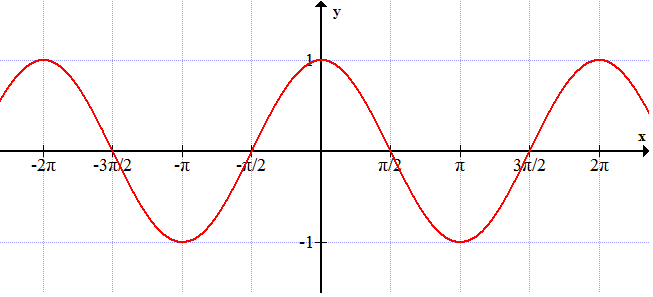
\includegraphics[scale=0.4]{projekt.png}
\caption{Wykres funkcji $\sin$}%
\end{figure}

\subsection{Funkcja logarytmiczna}
\begin{figure}[!ht]
\label{obrazek2}
\centering
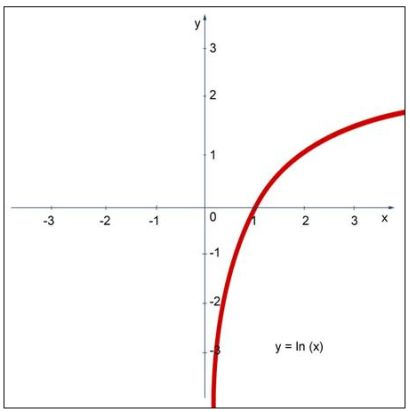
\includegraphics[scale=0.4]{funklog.jpg}
\caption{Wykres funkcji $y=\ln(x)$}%
\end{figure}

\begin{thebibliography}{9}
\bibitem{1}
  REGEL WIESŁAWA,
  \emph{ 81 zadań o funkcjach zespolonych z pełnymi rozwiązaniami krok po kroku}. Data wydania: 2014-05-23
\bibitem{2}
https://pl.wikipedia.org/wiki/Funkcja
\bibitem{3}
https://pl.wikipedia.org/wiki/Funkcja\_Dirichleta
\bibitem{4}
https://pl.wikipedia.org/wiki/Funkcja\_Riemanna
\end{thebibliography}


\end{document} 
